\documentclass[10pt,a4paper]{article}

\usepackage[utf8]{inputenc}
\usepackage[T1]{fontenc}
\usepackage[margin=2.1cm]{geometry}
\usepackage{graphicx}
\usepackage{booktabs}
\usepackage{tabularx}
\usepackage{array}
\usepackage{amsmath}
\usepackage{microtype}
\usepackage{caption}
\usepackage{subcaption}
\usepackage{hyperref}
\usepackage{xcolor}

\graphicspath{{plots/}}
\hypersetup{colorlinks=true,linkcolor=black,citecolor=black,urlcolor=blue}
\captionsetup{font=small,labelfont=bf}
\setlength{\parindent}{1.2em}
\setlength{\parskip}{0.25em}
\setlength{\emergencystretch}{2em}
\raggedbottom

\title{\vspace{-1.4cm}\textbf{FriendFeed: What Makes a Post Successful?}\\
\large Data Mining I Project Report}
\author{Group 60}
\date{September 2026}

\begin{document}

\maketitle
\vspace{-0.8cm}

\begin{abstract}
This project studies which combinations of post format, posting time, source service, and author characteristics are associated with unusually high engagement on FriendFeed. The raw dataset contains more than 66 million records from a two-month observation period in 2010. We constructed a post-level table, gave each post the same seven-day opportunity to collect reactions, and defined high engagement as at least seven likes or comments, corresponding to the observed 99th percentile. Association rule mining found that native FriendFeed posts were strongly overrepresented among highly engaged posts, especially when the author had 100--999 followers or the post contained an image. A reach-adjusted sensitivity analysis found a separate pattern for Bookmarklet posts from low-follower authors. MiniBatch K-means produced seven clusters, but the best silhouette score was only 0.120. The clustering therefore describes broad posting styles rather than clear natural groups. The findings are descriptive associations and should not be interpreted as causal effects.
\end{abstract}

\section{Introduction}

Online platforms contain large amounts of content, but attention is distributed very unevenly. Understanding which observable characteristics tend to occur together with engagement can help a publisher decide how and when to present content. It can also reveal whether apparent content effects are actually connected to the size of the author's existing audience. FriendFeed is useful for this question because the dataset combines posts, comments, likes, user profiles, external services, and social-network relationships rather than presenting an already prepared modelling table.

The research question is: \emph{Which combinations of post format, posting time, source, and author characteristics are associated with unusually high engagement on FriendFeed, and do these patterns remain after accounting for audience size?} This is a data-mining problem rather than a simple correlation question. The outcome is highly skewed, the information is spread across several large files, and potentially useful patterns involve combinations of categorical and numerical attributes. The work follows the knowledge-discovery process of understanding, cleaning, transforming, mining, and interpreting the data \cite{fayyad1996}.

Association rule mining is the main method because it returns statements that can be explained directly, such as a source service and follower band occurring together with high engagement. Clustering is used as a second, unsupervised view of the data. It asks whether posts form broader groups before engagement is examined. The two methods answer related but different questions: rules look for supported combinations connected to a defined outcome, while clustering looks for structure without using that outcome.

\section{Data and representation}

The FriendFeed dataset was collected from August 1 to September 30, 2010 and was distributed with the course. It originates from the study by Celli and colleagues \cite{celli2010}. The original files contain no header rows and use three different separators: tabs for entries, comments, likes, and following events; pipes for users and services; and commas for subscriptions. Table~\ref{tab:raw-data} shows the number of records successfully read from each source.

\begin{table}[ht]
\centering
\caption{Prepared records from the raw FriendFeed files.}
\label{tab:raw-data}
\begin{tabular}{lr}
\toprule
Table & Records \\
\midrule
Entries & 12,450,658 \\
Comments & 3,749,891 \\
Likes & 798,112 \\
Following events & 19,547,158 \\
Subscriptions & 27,811,816 \\
Services & 1,587,275 \\
Users & 671,840 \\
\bottomrule
\end{tabular}
\end{table}

The final representation has one row per post. Post identifiers and user identifiers are nominal attributes even though they are stored as text. Counts such as text length, followers, images, likes, and comments are ratio-scaled quantities. Source service and weekday are nominal, time-of-day bands are ordinal only in a loose cyclic sense, and media indicators are asymmetric binary attributes. Keeping these meanings explicit is important because an identifier must not be averaged and an unordered source category must not be treated as a number.

Engagement is the sum of likes and comments received during the first seven days after publication. A shared observation window prevents a post from appearing unsuccessful merely because it was observed for less time. Since comments end on September 30, posts published from September 24 onward do not have a complete seven-day window and are excluded from the main analysis. After this restriction and the timestamp checks, 10,868,872 posts from 246,332 authors remain eligible.

\section{Preprocessing pipeline}

The complete process is implemented as six numbered Python scripts and can be run with one command. The first stage reads every field as text with DuckDB and assigns explicit column names instead of relying on automatic detection. Empty strings, \texttt{\textbackslash N}, \texttt{null}, and \texttt{NULL} become missing values. Timestamps and counts are converted with safe casts, so a malformed value is flagged rather than stopping the complete run. Quotation marks are treated as ordinary text because the source files use delimiters but do not consistently apply CSV quoting.

The quality checks found no missing required identifiers. There were 13,282 entry timestamps and 130,995 comment timestamps outside the study window, mainly sentinel dates such as 1970. These rows remain auditable in the clean tables but are not used in time-dependent analysis. Fifty-nine service records had a structurally incorrect number of pipe-separated fields. They were written to a reject report rather than silently discarded. The typed tables were stored as Zstandard-compressed Parquet. This reduced repeated parsing work and allowed DuckDB to read only the columns required by later queries.

The second stage deduplicates post identifiers and aggregates before joining. Comments and likes are first counted by post, while subscriptions are counted in both directions to obtain approximate follower and following counts. Aggregating first avoids a many-to-many join in which every like could be multiplied by every comment. The subscription file is interpreted as subscriber followed by subscribed-to account. This direction is recorded as a project assumption because the supplied documentation is incomplete for that table.

The third stage joins the post, engagement, and author aggregates. HTML tags are removed before calculating character and word counts. Additional features include hashtag count, URL count, image and video indicators, posting hour, weekday, source service, author activity, connected-service count, follower count, and following count. The twenty most common sources are retained and all remaining sources are grouped as ``Other.'' Full post text, profile names, descriptions, and external URLs are left out of the analysis table because the selected methods do not require them.

The engagement distribution required a careful threshold choice. At the 90th percentile the discrete threshold was one interaction, which would make ``high engagement'' mean only that somebody reacted. The 99th percentile was therefore used. It corresponds to at least seven likes or comments in seven days and marks 115,330 posts, or 1.061\% of the eligible data, as highly engaged. Reach-adjusted engagement is defined as engagement divided by followers plus one and is calculated only when the follower snapshot contains the author. Its high threshold is 0.5, obtained from the 99th percentile among posts with positive reach-adjusted engagement.

\section{Exploratory analysis}

The outcome is extremely right-skewed. Of the eligible posts, 9,670,357 received no interaction, 906,117 received exactly one, 177,068 received between two and six, and 115,330 received seven or more. The mean was 0.334 interactions, while the maximum was 2,583. Figure~\ref{fig:distribution} uses a logarithmic vertical scale so both the mass at zero and the long tail are visible.

\begin{figure}[ht]
\centering
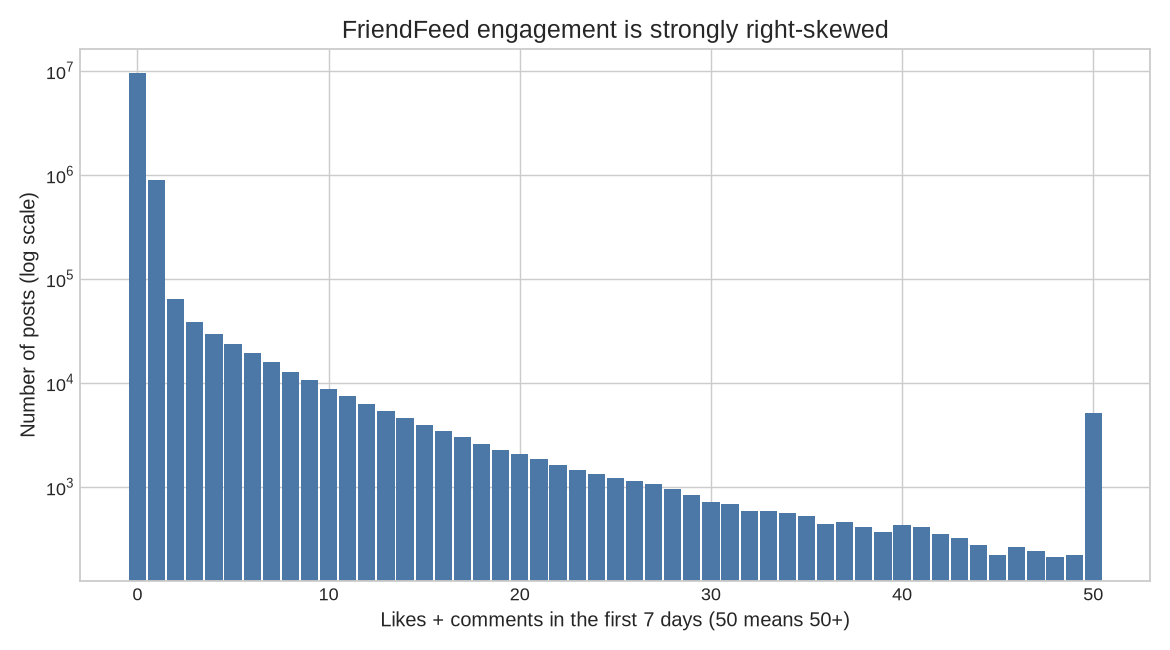
\includegraphics[width=0.82\linewidth]{engagement_distribution.png}
\caption{Distribution of seven-day engagement. The last bar combines values of 50 or more.}
\label{fig:distribution}
\end{figure}

Source service has a strong descriptive relationship with the outcome. Native FriendFeed posts have a 9.52\% high-engagement rate, compared with the overall baseline of 1.061\%. Bookmarklet posts have a rate of 2.22\%, while Twitter posts have a rate of 0.46\%. Some large automated sources, particularly Ping.fm, rarely reach the threshold. Figure~\ref{fig:source} makes this imbalance clear. Source is likely capturing several mechanisms at once, including content type, automatic cross-posting, and the audience that used each service.

\begin{figure}[ht]
\centering
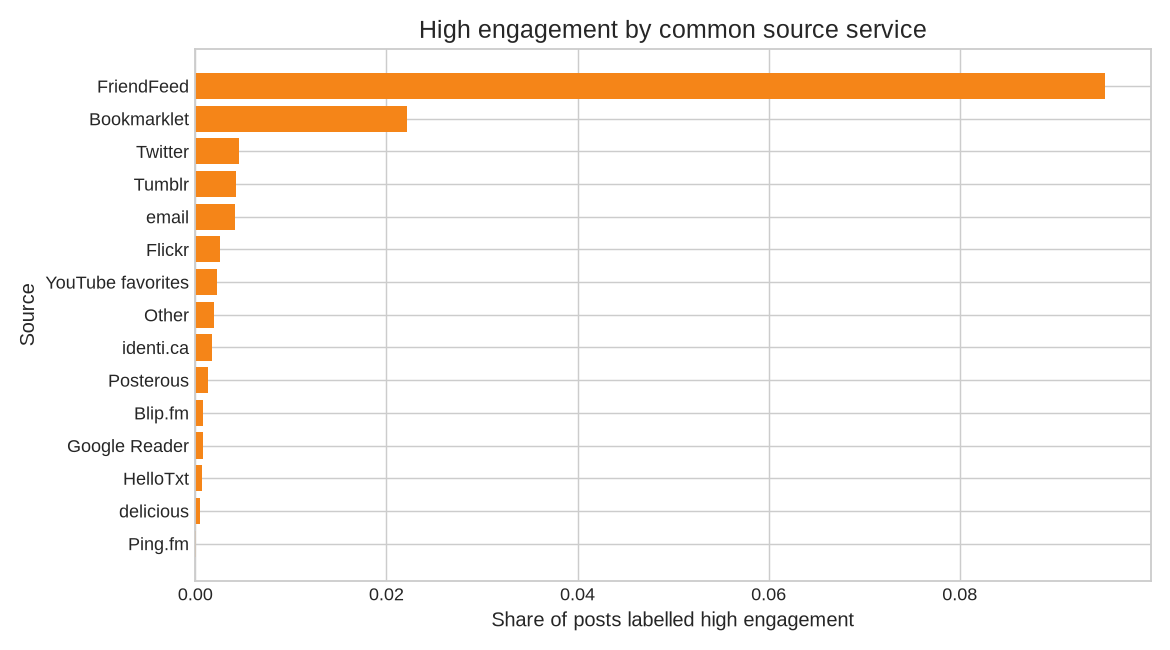
\includegraphics[width=0.82\linewidth]{high_engagement_by_source.png}
\caption{Share of posts reaching at least seven interactions for common source services.}
\label{fig:source}
\end{figure}

Author reach is an important confounder. The high-engagement share rises from 0.018\% for authors with 1--9 recorded followers to 3.26\% for 100--999 followers and 3.70\% for at least 1,000 followers. Posts with unknown follower counts have a rate of 1.34\%, showing why unknown values cannot be treated as zero. Posting hour also varies with the outcome. The rate is lowest around 02:00--04:00 and highest around 20:00, in the dataset's GMT+1 time zone. These are unadjusted comparisons and may partly reflect differences in source and audience composition.

\begin{figure}[ht]
\centering
\begin{subfigure}[t]{0.49\linewidth}
\centering
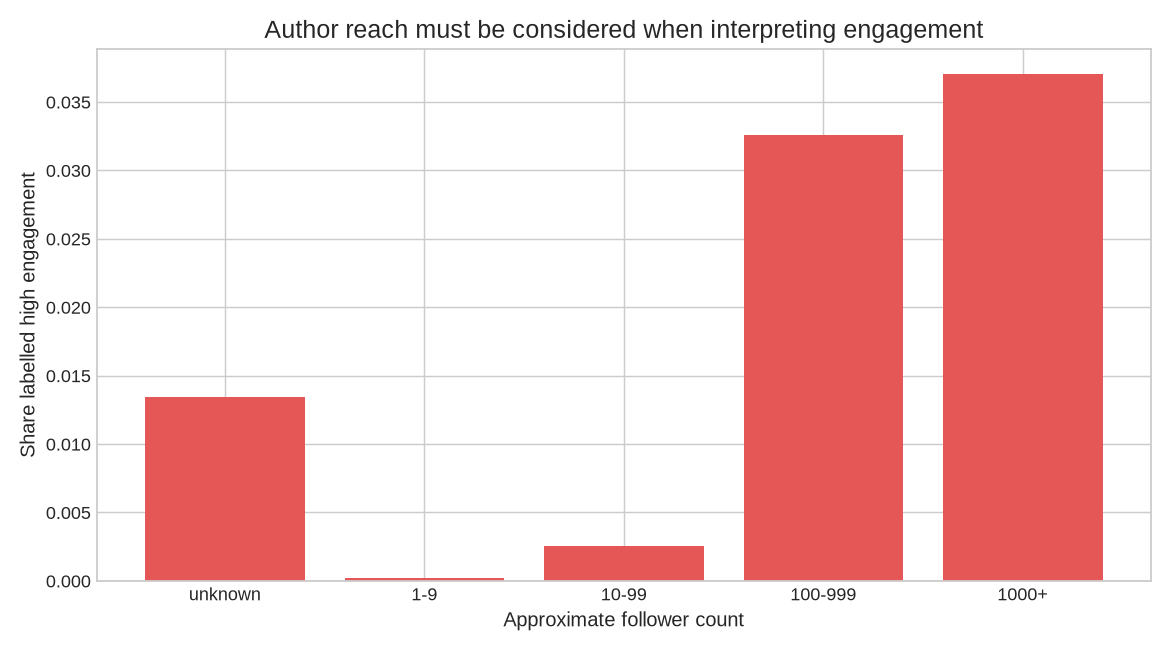
\includegraphics[width=\linewidth]{high_engagement_by_followers.png}
\caption{Approximate follower count.}
\end{subfigure}
\hfill
\begin{subfigure}[t]{0.49\linewidth}
\centering
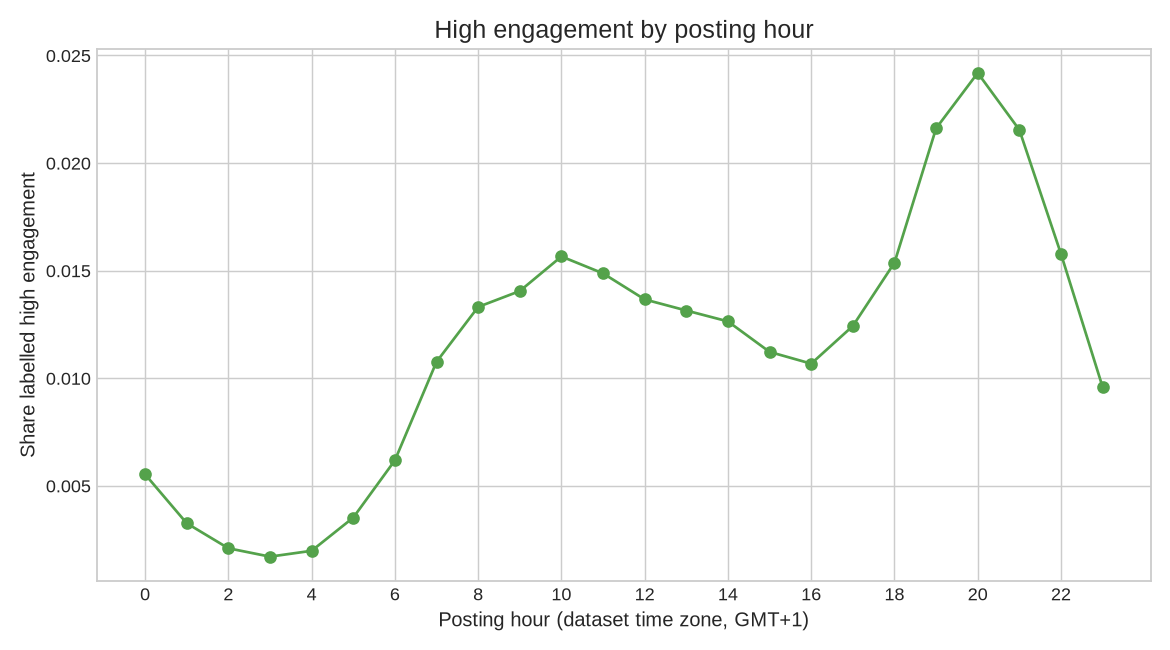
\includegraphics[width=\linewidth]{high_engagement_by_hour.png}
\caption{Posting hour in GMT+1.}
\end{subfigure}
\caption{High-engagement shares by author reach and posting time.}
\label{fig:reach-time}
\end{figure}

\section{Association rule mining}

Each post was converted to a small transaction of categorical items. The items describe post-length band, time of day, weekday, source group, follower band, author-activity band, image presence, video presence, and weekend status. The consequent is the high-engagement item. Antecedents of one or two items were counted over all 10.87 million eligible posts. A rule was retained when it had at least 500 antecedent records, support of at least 0.001, confidence of at least 0.10, and lift above 1.05.

For an antecedent $X$ and the high-engagement item $H$, the measures are
\begin{equation}
\operatorname{support}(X\Rightarrow H)=\frac{N(X\cap H)}{N},\qquad
\operatorname{confidence}(X\Rightarrow H)=\frac{N(X\cap H)}{N(X)},
\end{equation}
\begin{equation}
\operatorname{lift}(X\Rightarrow H)=
\frac{\operatorname{confidence}(X\Rightarrow H)}{\operatorname{support}(H)}.
\end{equation}
Confidence measures how often the consequent occurs when the antecedent occurs, while lift compares that confidence with the overall 1.061\% baseline. Lift is essential here because high engagement is rare; confidence without a baseline can be misleading \cite{tan2019}.

Nine rules passed the thresholds. Table~\ref{tab:rules} shows the strongest and most informative examples. The leading rule combines native FriendFeed posting with 100--999 followers. It covers 229,431 posts, of which 54,685 are highly engaged. Its confidence is 23.84\% and its lift is 22.46, meaning the outcome is about twenty-two times as common as in the eligible population. Native FriendFeed posts with an image also have high confidence and strong support. The repeated presence of \texttt{source=FriendFeed} indicates that source is the dominant feature in the retained rules.

\begin{table}[ht]
\centering
\caption{Selected rules for raw high engagement. Support and confidence are percentages.}
\label{tab:rules}
\small
\begin{tabularx}{\linewidth}{>{\raggedright\arraybackslash}X r r r}
\toprule
Antecedent $X$ & Support & Confidence & Lift \\
\midrule
FriendFeed source and 100--999 followers & 0.503 & 23.84 & 22.46 \\
FriendFeed source and image present & 0.280 & 20.65 & 19.46 \\
FriendFeed source and 100--999 author posts & 0.577 & 13.61 & 12.82 \\
Evening and FriendFeed source & 0.282 & 13.27 & 12.51 \\
Short post and FriendFeed source & 0.418 & 11.13 & 10.49 \\
\bottomrule
\end{tabularx}
\end{table}

The reach-adjusted sensitivity analysis is stricter because authors without follower information are not assigned a score. One rule passed the same evidence thresholds: Bookmarklet source together with 1--9 followers. It covers 91,791 posts, has support 0.139\%, confidence 16.41\%, and lift 37.53 relative to the adjusted-target baseline of 0.437\%. This pattern differs from the raw rules and shows that raw popularity and engagement relative to a small audience are not the same concept.

\section{Clustering}

Clustering was performed without engagement, likes, or comments as input. Numerical features were transformed with $\log(1+x)$ where needed and standardized. Posting hour was represented by sine and cosine values so that 23:00 is close to 00:00. Source, weekday, image presence, and video presence were one-hot encoded. A deterministic hash sample of 100,000 eligible posts kept computation manageable while remaining large enough to describe common behaviour.

MiniBatch K-means was fitted for two through eight clusters. The number of clusters was chosen by the largest silhouette score on a fixed 5,000-post evaluation sample \cite{rouseeuw1987,sculley2010}. Seven clusters gave the highest score, 0.120, as shown in Figure~\ref{fig:silhouette}. This value is low and the alternatives are close, so there is weak evidence for sharply separated groups. The clusters should be read as a compact description of recurring post styles, not as objectively distinct types of FriendFeed users.

\begin{figure}[ht]
\centering
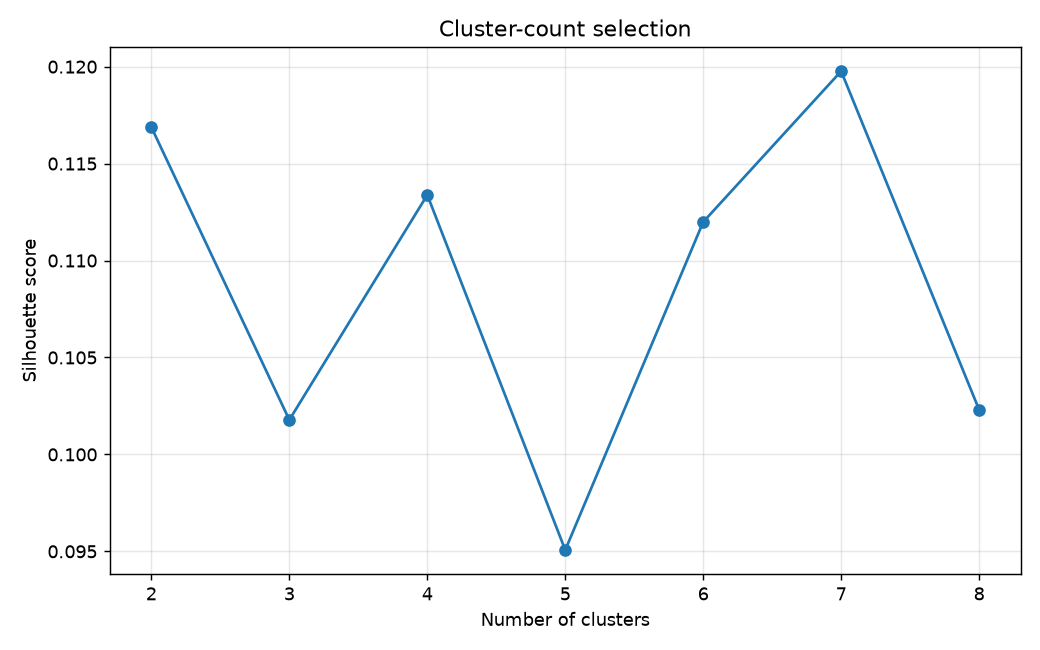
\includegraphics[width=0.66\linewidth]{cluster_silhouette.png}
\caption{Silhouette score used to compare candidate cluster counts.}
\label{fig:silhouette}
\end{figure}

Table~\ref{tab:clusters} summarizes the profiles after engagement was joined back for interpretation. The two largest clusters contain posts with URLs and differ mainly in time and author characteristics; both have below-baseline high-engagement shares. Clusters 0 and 3 contain posts with almost no URLs and have much higher high-engagement shares. Cluster 4 is associated with authors having more followers and connected services. Clusters 5 and 6 are distinguished by heavier hashtag use. These profiles support the exploratory conclusion that source and author context matter, but their overlap confirms that post characteristics do not form cleanly separated populations.

\begin{table}[ht]
\centering
\caption{Interpretation of the seven-cluster solution.}
\label{tab:clusters}
\small
\begin{tabularx}{\linewidth}{c r >{\raggedright\arraybackslash}X r}
\toprule
Cluster & Posts & Main profile & High share \\
\midrule
0 & 8,644 & Twitter mode, almost no URLs & 5.44\% \\
1 & 27,158 & Other-source mode, URLs common, later-day pattern & 0.22\% \\
2 & 28,955 & Other-source mode, URLs common, early-hour pattern & 0.05\% \\
3 & 7,389 & Short Twitter-style posts, almost no URLs & 4.82\% \\
4 & 20,149 & More followers and connected services & 0.63\% \\
5 & 2,244 & Hashtag-heavy Twitter-style posts & 0.13\% \\
6 & 5,461 & Moderate hashtag use, Twitter mode & 0.77\% \\
\bottomrule
\end{tabularx}
\end{table}

\section{Discussion and limitations}

The most consistent result is that native FriendFeed activity behaves differently from automatically imported content. This does not show that choosing FriendFeed as a source causes engagement. Native posts may be created by more active users, may be shown differently by the platform, or may reach audiences with different habits. The association rules describe combinations that are common enough to examine and unusually connected to the target, but they do not isolate a causal mechanism.

Audience size is another major limitation. The follower table is a static snapshot collected after the posting period, so it is only an approximation of reach at publication time. About 1.41 million eligible posts have no follower count in that snapshot. The reach-adjusted analysis keeps those values missing, but the remaining ratio is still crude: follower count does not measure how many people actually saw a post, and dividing by followers plus one can favour very small accounts. The adjusted result should therefore be treated as a sensitivity check rather than a definitive engagement rate.

The seven-day window improves comparability but misses reactions arriving later. Likes and comments are also given equal weight even though they require different effort. The analysis uses structural text features rather than language or meaning, which avoids unreliable multilingual sentiment processing but leaves topic effects unexplored. External service categories can also encode automated posting behaviour. Finally, the low silhouette score shows that the chosen clustering features do not create strong natural groups. Reporting that weak result is preferable to claiming clusters that the evidence does not support.

Reliability was addressed by retaining quality flags, logging malformed source lines, using all eligible posts for rule counts, recording random seeds, and separating outcome construction from clustering inputs. The complete process is reproducible from the raw files with the numbered scripts. A useful extension would be a chronological analysis that constructs author activity and follower information only from data available before each post. That would better support prediction, although it would still not establish causality.

\section{Conclusion}

The project transformed a 7.1 GB multi-table social-network dataset into a reproducible post-level mining process. High engagement is rare: only 1.061\% of posts receive at least seven reactions in seven days. Association rules show that native FriendFeed source, moderate-to-large audience size, image presence, and some timing and activity combinations are strongly associated with this outcome. The reach-adjusted result highlights a different pattern for Bookmarklet posts from low-follower authors. Clustering finds several broad posting styles, but their low silhouette scores show substantial overlap. The practical conclusion is therefore modest: source and author context are useful for identifying where engagement is concentrated, but the data does not justify a simple claim that one post feature makes content successful.

\begin{thebibliography}{9}

\bibitem{celli2010}
F. Celli, F. Marta L. Di Lascio, M. Magnani, B. Pacelli, and L. Rossi.
\newblock Social network data and practices: the case of FriendFeed.
\newblock In \emph{International Conference on Social Computing, Behavioral Modeling and Prediction}, Springer, 2010.

\bibitem{fayyad1996}
U. Fayyad, G. Piatetsky-Shapiro, and P. Smyth.
\newblock From data mining to knowledge discovery in databases.
\newblock \emph{AI Magazine}, 17(3):37--54, 1996.

\bibitem{rouseeuw1987}
P. J. Rousseeuw.
\newblock Silhouettes: a graphical aid to the interpretation and validation of cluster analysis.
\newblock \emph{Journal of Computational and Applied Mathematics}, 20:53--65, 1987.

\bibitem{sculley2010}
D. Sculley.
\newblock Web-scale k-means clustering.
\newblock In \emph{Proceedings of the 19th International Conference on World Wide Web}, pages 1177--1178, 2010.

\bibitem{tan2019}
P.-N. Tan, M. Steinbach, A. Karpatne, and V. Kumar.
\newblock \emph{Introduction to Data Mining}, second edition.
\newblock Pearson, 2019.

\end{thebibliography}

\end{document}
